%% For double-blind review submission
\documentclass[sigplan,10pt,review,anonymous]{acmart}\settopmatter{printfolios=true}
%% For single-blind review submission
%\documentclass[sigplan,10pt,review]{acmart}\settopmatter{printfolios=true}
%% For final camera-ready submission
%\documentclass[sigplan,10pt]{acmart}\settopmatter{}

%% Note: Authors migrating a paper from traditional SIGPLAN
%% proceedings format to PACMPL format should change 'sigplan' to
%% 'acmsmall'.


%% Some recommended packages.
\usepackage{booktabs}   %% For formal tables:
                        %% http://ctan.org/pkg/booktabs
\usepackage{subcaption} %% For complex figures with subfigures/subcaptions
                        %% http://ctan.org/pkg/subcaption

\usepackage{amssymb}
\setcounter{tocdepth}{3}
\usepackage{graphicx}
\usepackage{listings,calc}
%\usepackage{subcaption}
%\captionsetup{compatibility=false}

\lstset{language=Java, numbers=left, mathescape, columns=fullflexible, keepspaces=true, tabsize=2, basicstyle=\lst@ifdisplaystyle\scriptsize\fi}

\usepackage{url}

\makeatletter\if@ACM@journal\makeatother
%% Journal information (used by PACMPL format)
%% Supplied to authors by publisher for camera-ready submission
\acmJournal{PACMPL}
\acmVolume{1}
\acmNumber{1}
\acmArticle{1}
\acmYear{2017}
\acmMonth{1}
\acmDOI{10.1145/nnnnnnn.nnnnnnn}
\startPage{1}
\else\makeatother
%% Conference information (used by SIGPLAN proceedings format)
%% Supplied to authors by publisher for camera-ready submission
\acmConference[PL'17]{ACM SIGPLAN Conference on Programming Languages}{January 01--03, 2017}{New York, NY, USA}
\acmYear{2017}
\acmISBN{978-x-xxxx-xxxx-x/YY/MM}
\acmDOI{10.1145/nnnnnnn.nnnnnnn}
\startPage{1}
\fi


%% Copyright information
%% Supplied to authors (based on authors' rights management selection;
%% see authors.acm.org) by publisher for camera-ready submission
\setcopyright{none}             %% For review submission
%\setcopyright{acmcopyright}
%\setcopyright{acmlicensed}
%\setcopyright{rightsretained}
%\copyrightyear{2017}           %% If different from \acmYear


%% Bibliography style
\bibliographystyle{ACM-Reference-Format}
%% Citation style
%% Note: author/year citations are required for papers published as an
%% issue of PACMPL.
%\citestyle{acmauthoryear}  %% For author/year citations
%\citestyle{acmnumeric}     %% For numeric citations
%\setcitestyle{nosort}      %% With 'acmnumeric', to disable automatic
                            %% sorting of references within a single citation;
                            %% e.g., \cite{Smith99,Carpenter05,Baker12}
                            %% rendered as [14,5,2] rather than [2,5,14].
%\setcitesyle{nocompress}   %% With 'acmnumeric', to disable automatic
                            %% compression of sequential references within a
                            %% single citation;
                            %% e.g., \cite{Baker12,Baker14,Baker16}
                            %% rendered as [2,3,4] rather than [2-4].



\begin{document}

%% Title information
\title[Java Library]{A Java Library for Actor-Based Cooperative Scheduling}         %% [Short Title] is optional;
                                        %% when present, will be used in
                                        %% header instead of Full Title.
%\titlenote{with title note}             %% \titlenote is optional;
                                        %% can be repeated if necessary;
                                        %% contents suppressed with 'anonymous'
%\subtitle{Subtitle}                     %% \subtitle is optional
%\subtitlenote{with subtitle note}       %% \subtitlenote is optional;
                                        %% can be repeated if necessary;
                                        %% contents suppressed with 'anonymous'


%% Author information
%% Contents and number of authors suppressed with 'anonymous'.
%% Each author should be introduced by \author, followed by
%% \authornote (optional), \orcid (optional), \affiliation, and
%% \email.
%% An author may have multiple affiliations and/or emails; repeat the
%% appropriate command.
%% Many elements are not rendered, but should be provided for metadata
%% extraction tools.

%% Author with single affiliation.
\author{Vlad Serbanescu}
\authornote{with author1 note}          %% \authornote is optional;
                                        %% can be repeated if necessary
\orcid{nnnn-nnnn-nnnn-nnnn}             %% \orcid is optional
\affiliation{
  \position{PhD Student}
  \department{Formal Methods}              %% \department is recommended
  \institution{Centrum Wiskunde \& Informatica}            %% \institution is required
  \streetaddress{Science Park 123}
  \city{Amsterdam}
  \state{State1}
  \postcode{Post-Code1}
  \country{Netherlands}
}
\email{vlad.serbanescu@cwi.nl}          %% \email is recommended

%% Author with two affiliations and emails.
\author{Frank de Boer}
\authornote{with author2 note}          %% \authornote is optional;
                                        %% can be repeated if necessary
\orcid{nnnn-nnnn-nnnn-nnnn}             %% \orcid is optional
\affiliation{
  \position{Professor}
  \department{Formal Methods}              %% \department is recommended
  \institution{Centrum Wiskunde \& Informatica}            %% \institution is required
  \streetaddress{Science Park 123}
  \city{Amsterdam}
  \state{State1}
  \postcode{Post-Code1}
  \country{Netherlands}
}
\email{frank.s.de.boer@cwi.nl}         %% \email is recommended


\author{Mahdi Jaghouri}
\authornote{with author1 note}          %% \authornote is optional;
%% can be repeated if necessary
\orcid{nnnn-nnnn-nnnn-nnnn}             %% \orcid is optional
\affiliation{
  \department{Formal Methods}              %% \department is recommended
  \institution{Centrum Wiskunde \& Informatica}            %% \institution is required
  \streetaddress{Science Park 123}
  \city{Amsterdam}
  \state{State1}
  \postcode{Post-Code1}
  \country{Netherlands}
}
\email{jaghouri@cwi.nl}         %% \email is recommended


%% Paper note
%% The \thanks command may be used to create a "paper note" ---
%% similar to a title note or an author note, but not explicitly
%% associated with a particular element.  It will appear immediately
%% above the permission/copyright statement.
\thanks{with paper note}                %% \thanks is optional
                                        %% can be repeated if necesary
                                        %% contents suppressed with 'anonymous'


%% Abstract
%% Note: \begin{abstract}...\end{abstract} environment must come
%% before \maketitle command
\begin{abstract}
In this paper we introduce  and evaluate a new actor-based library in Java with a scalable implementation of cooperative scheduling of messages within an actor.
This allows for multiple entry points for suspending and resuming execution while processing a message.
By means of a typical benchmark we evaluate our proposed solution and compare it
to other thread-based implementations of cooperative scheduling.
\end{abstract}


%% 2012 ACM Computing Classification System (CSS) concepts
%% Generate at 'http://dl.acm.org/ccs/ccs.cfm'.
%\begin{CCSXML}
%<ccs2012>
%<concept>
%<concept_id>10011007.10011006.10011008</concept_id>
%<concept_desc>Software and its engineering~General programming languages</concept_desc>
%<concept_significance>500</concept_significance>
%</ccs2012>
%\end{CCSXML}
%
%\ccsdesc[500]{Software and its engineering~General programming languages}
%\ccsdesc[300]{Social and professional topics~History of programming languages}
%% End of generated code


%% Keywords
%% comma separated list
\keywords{Actors, Cooperative Scheduling, Functional Programming, Object-Orientation, Java Library,Scala}  %% \keywords is optional


%% \maketitle
%% Note: \maketitle command must come after title commands, author
%% commands, abstract environment, Computing Classification System
%% environment and commands, and keywords command.
\maketitle

\section{Introduction}

%how this scala library is build up
%compiler which translates to scala making use of features for the functional part, source-to-source translation
%underlying java library iwth the thread model
%this compiler supports the FLI

%the actor-based model smotthly integrates with scala

The Actor-based model of computation~\cite{Agha} is particularly tailored to the description of distributed systems. 
Actors represent processes that execute in parallel and interact via asynchronous communication of messages. 
The Abstract Behavioral Specification (ABS)~\cite{abs} Language has been developed for modeling parallel and distributed systems based on the actor model and provides extensive support for formal analysis like functional analysis~\cite{KeY}, resource analysis~\cite{saco} and deadlock analysis~\cite{dead}. Syntactically ABS has a similar structure to Java and Scala languages, offering both functional and object-oriented support.
In this paper, we bring the concepts and advantages of ABS to programming level by implementing a library that can be directly used from Scala and Java. Our solution uses an underlying thread model implemented in Java to support a very powerful feature of ABS, namely cooperative scheduling. Together with this model we provide a source-to-source translation from ABS to Scala to support both the object-oriented and functional programming paradigms of ABS. Most importantly the library has support for a Foreign Language Interface (FLI) that offers ABS as an extension of the Scala language which provides a new concurrency model and corresponding analysis techniques.
% e.g., recent developments have focused on the modeling and analysis of Cloud applications~\cite{Albert}. 


\par In ABS, asynchronous messages are modeled as methods of an actor.
Sending an asynchronous message will schedule the execution of the corresponding method in the callee, returning immediately a future that, upon completion, will hold the result of the method execution, or in case of errors, the thrown exception.
This ``programming to interfaces'' paradigm enables static type checking of message passing at compile time.
This is contrast to the typical approach in Scala where messages are allowed to have any type and thus are only checked at run-time whether the receiver can handle them.

ABS further extends the Actor-based model with a high-level synchronization mechanism that allows actors to suspend in a cooperative manner the execution of the current message and start another queued message. 
The continuation of the suspended message, which is automatically put back in the message queue, may also be assigned an enabling condition. 
A typical use case is awaiting the completion of a future in the same method that has sent the corresponding message.
This simplifies the programming logic by enabling the programmer to process the outcome of an asynchronous method call in the same place where it was sent (in a way similar to dealing with synchronous calls).
Bear in mind that the continuation will be executed in the same actor thread thus (unlike the {\ttfamily onComplete} hooks in Scala that may run in a different thread) pose no threat to actor semantics.
%More details on syntax and behavior of ABS is presented in Section \ref{}. % section 2

%In this paper we introduce and evaluate a new run-time system in Java for the use of ABS as a full-fledged programming language. 
%As such our run-time system allows a component-based design in Java when following the ABS programming methodology.
The main challenge is the development of an efficient and scalable source-to-source implementation of cooperative scheduling. 
%which, in the presence of synchronous calls, gives rise to the suspension of the entire call stack generated from a message.
%The continuation of the suspended message including the stack frame needs to be saved in order for execution to resume properly once the message is rescheduled.
The basic feature of our proposed solution is the implementation of messages by means of lambda expressions (as provided by Java 8), i.e., the method call specified in a message
is translated into a corresponding lambda expression~\cite{lambdas} which is passed and stored as
an object of type Callable or Runnable (depending on whether it returns a result). We show how this basic feature is extended in the presence of synchronous calls that give rise to the suspension of the entire call stack generated from a message.

We describe how we implemented ABS actors and cooperative scheduling using Java thread pools and executor services.  
As elaborated in Section \ref{bench}, we took an approach with negligible performance penalties regarding message passing and cooperative scheduling. 
We describe step by step how to support up to millions of messages,  actors, and suspended continuations.


%This feature forms the basis of a run-time system which manages
%the sending, storage and execution of the messages and their continuations
%which arise because of the cooperative scheduling.
By means of a typical benchmark we evaluate our proposed solution and compare it
to other thread-based implementations in Java or Erlang(a language that uses lightweight threads) of cooperative scheduling.


%related work takka.
% the original version of Akka did not support it, but a recent version provides a first approach to programming to interfaces Takka.
\paragraph{Related Work.} 
Our main motivation is a Scala implementation of the ABS language as a full-fledged Actor-based programming language which fully supports the "programming to interfaces'' paradigm. 
In contrast, Java libraries for programming actors like Akka~\cite{Akka} mainly provide pure asynchronous message passing which does not support the use of application programming interfaces (API) because, for example, in Akka/Java a message is only typed as a Java Object, so there is no static typing of messages, nor are they part of the actor interface.  A first approach for supporting programming to interfaces was proposed in Takka library~\cite{takka}. 
Distinguishing features of the ABS comprise of high-level constructs for cooperative scheduling which allow the application of formal methods, e.g.,
formal analysis of deadlock~\cite{deadlock}.
The Actor model in Scala~\cite{Scala} does provide a suspension mechanism, but its use is \emph{not} recommended because it actually blocks the whole thread and causes
%its intricate semantics and 
degradation of performance.
It is possible to register a {\em continuation} piece of code to run upon completion of a future, but that may run in a separate thread which however breaks the actor semantics and may cause race conditions inside the actor.

There exist various implementation attempts for cooperative scheduling in ABS.
The approach followed in the Java backend of ABS~\cite{abs,Schafer} and in the Erlang backend~\cite{Erlang} is process-oriented in the sense that sending a message is implemented by the generation of a corresponding process. We will compare these backends with our solution in Java which allows to store messages (as objects of type Callable or Runnable) before executing them (data-oriented).

The focus of our paper is on an efficient implementation of cooperative scheduling in Java.
Implementations in other languages allow for different approaches:
In the Haskell backend for ABS~\cite{Haskell}, for example, the use of continuations allows
to queue a message as a process and dequeue it for execution and the C implementation of cooperative scheduling for the
Encore language~\cite{Encore} uses low-level (e.g., machine code) operations for
storing and retrieving call stacks from memory.

In contrast, in the Actor-based modeling language Rebeca~\cite{Sirjani}, for example,
messages are queued and processed in a run-to-completion mode of execution.
Cooperative scheduling is a powerful means for the expression and analysis
of fine-grained run-time dependencies between messages.

The rest of this paper is organized as follows: In Section~\ref{lang} we give an overview of the main features that the target actor-based model has. Section~\ref{scheme} presents how our solution transitions from a process-oriented approach to a data-oriented approach. Section~\ref{run} describes the implementation the run-time system for the actor-based model. In Section~\ref{bench} we show the experimental evaluation of our solution followed by the conclusions drawn in Section~\ref{conc}.









\section{ABS Language Concepts}
\label{lang}
%Our reference modeling language for analyzing cooperative scheduling is ABS \cite{abs}, an actor-based modeling language whose semantics offers high-level synchronization mechanisms for parallel and distributed applications. This is a very powerful modeling language with extensive support for concurrent programming \cite{cog}, resource analysis \cite{saco}, deadlock analysis \cite{dead} and remote communication \cite{dis,cloud}. ABS provides high-level constructs for modeling asynchronous communication between actors using messages and cooperative scheduling of these messages by an actor.
%Mahdi:
%{\bfseries the following are not the `focus of this paper' as suggested in the previous sentence}
%These constructs can have optional annotations that define custom schedulers in order to model an actor's specific behavior. Asynchronous method calls can also be annotated with costs and deadlines which can be combined with cooperative scheduling policies to create a very powerful scheduler.
In this section we informally describe the main features of the flow of control
underlying the semantics of cooperative scheduling in the ABS language.
For a detailed description of the syntax of the ABS language we refer to~\cite{abs}.

\subsection{Method Invocations}\label{amc}
Abstracting from the syntax of the actual parameters,
in ABS an asynchronous invocation of a method \lstinline|m| of an actor \lstinline|a| is described by a statement
\lstinline|Future f=a!m()|, where f is a future used to store the return value
(asuming that m contains a return statement).
In our backend this invocation will be stored in a queue of the called actor a.
Futures can be passed around as references and provide a get operation
described by \lstinline|f.get| which results in the value returned and blocks
the current process if the corresponding method invocation has not yet computed
the return value.

Again abstracting from the syntax of the actual parameters,
ABS additionally features synchronous method calls described in the standard manner
by statements of the form \lstinline| x=a.m()| (also assuming here that the method m returns a value). In case the called actor \lstinline|a| belongs to a different 
COG (i.e., Concurrent Object Group which shares one thread of control, see~\cite{abs})
than the caller the semantics of such a synchronous call can be translated
by \lstinline|Future f=a!m(); x= f.get|, for some future f (of the appropriate type).
In case the called actor \lstinline|a |and the caller belong to the same COG such a synchronous call can be translated by \lstinline|Future f=a!m( ); x= f.get;resume|,
where the auxiliary statement \lstinline|resume| (as introduced in~\cite{resume})
is implememted in our Java backend by a specific scheduling policy which preserves the synchronous call stack.
This will be described in more detail in Section~\ref{run}.


%The semantics of ABS allows for synchronous method calls of the form \lstinline|a.m()| or \lstinline|this.m()|. These calls have to block the callee actor until they return. Actors also communicate with each other using asynchronous method invocation. This is written as \lstinline|a!m()| or \lstinline|this.m()| which sends a message to an actor to execute method \lstinline|m()|. The callee actor can then proceed with its execution without blocking. Each ABS actor has a queue that stores all asynchronous invocations coming from other actors as messages and executes them sequentially. An important observation to make here is that in modeling an application, ABS assumes there is no "message overtaking", that is the order of messages delivered from one particular actor to another is the same as the order in which they were generated. The result of a message execution can be captured in an future which the caller actor can use to retrieve the result, but also to block its current execution using \lstinline|f.get| in order to synchronize with the actor completing the future. One may also send the future as parameter of a message, allowing other actors to synchronize and use the results. ABS also has support for grouping Actors intoc and only actors belonging to the same group can communicate synchronously. The semantics of ABS allow this behavior as a call \lstinline|a.m()| can be translated as \lstinline|Future f=a!m(); f.get|. The only issue appears when we have a call like \lstinline|this.m()| as such a translation would result in a deadlock for the actor. In order to have a solution, we will first explain the second language concept of ABS.
%The semantics additionally allows for synchronous method calls that only change the internal state of an actor $\leftarrow$ {\bfseries what does this mean?}. 


%but for the scope of our analysis and implementation simplicity we will assume that each actor is defined in its own group. <-- then I would drop it from here


%The result of an asynchronous method invocation can be captured in an future which the caller actor can use to retrieve the result, but also to block its current execution in order to synchronize with the% callee actor. 
%This is done through the ``future.get" statement that a future supplies. % and has the same semantics as futures in other modeling and programming languages. 


%This is a constraint that our implementation needs to take into account and a synchronization mechanism as will be described in our modeled application later in this section $\leftarrow$ {\bfseries do we? make sure it is not overemphasized here.}. 


\subsection{Await Construct}
In ABS a statement of the form \lstinline|await f?|
suspends the executing process which can only be rescheduled if the method
invocation corresponding to the future \lstinline|f| has computed the return value.
Similarly, a statement of the form \lstinline|await b|, where \lstinline|b| denotes a boolean expression, suspends the executing process which can only be rescheduled if \lstinline|b| evaluates to true. In both cases the executing process is suspended and another (enabled) process (belonging to the same actor, or more generally, to the same COG) can be scheduled for execution.
In contrast, a statement like \lstinline|f.get| does not allow the scheduling of
another process of the same actor (COG). It thus blocks the entire actor (COG). Listing~\ref{ex} sketches a pattern of method definitions which gives rise to a suspended stack of synchronous calls; assume an asynchronous call to \lstinline|m1|; this may generate a synchronous call to \lstinline|m2| and subsequently this invocation may suspend on the future f. The main challenge addressed in this paper is to have an efficient implementation of such a suspended stack of synchronous calls.

%=======
%The "await" statement of ABS offers a high level mechanism that controls execution within an actor based on its internal state or the availability of the result of an asynchronous call via futures. A statement like \lstinline|await future?| differs from "future.get" as it does not block the entire execution of the actor, but instead blocks the current message from which the "await" statement was called and allows the actor to continue with executing other messages that are available in its queue. Similarly, for example \lstinline|await this.boolVar| will suspend the current message executing this statement until the field boolVar is set to true (while another method is being executed). In both uses of the "await" construct the suspended message will be made available once the future is completed or the boolean condition evaluates to true. Now we have a simple solution for translating \lstinline|this.m()| without creating a deadlock by translating it to \lstinline|Future f=a!m(); await f?|, but we still need to preserve the logic and resume from this point once \lstinline|m()| has completed. The basic non-deterministic scheduling policy does not guarantee this unless at the semantic level there is a specific contruct\cite{creol,resume}. The sketch of such a scenario is given in Listing \ref{ex}. 
%
\begin{lstlisting}[caption=ABS Example, label=ex]
	m1( ){
		...;
		this.m2( );
		...	//continuation of m1 <=>$C(m_1)$
	}

	m2( ){
		...
		await f?
		.... //continuation of m2 <=>$C(m_2)$
	}
\end{lstlisting}
%>>>>>>> Stashed changes



%The "await" statement of ABS offers a high level mechanism that controls execution within an actor (or, more generally, a COG) based on its internal state or the availability of the result of an asynchronous call via futures. A statement like \lstinline|await future?| differs from "future.get" 
%
%as it does not block the entire execution of the actor, but instead blocks the current message from which the "await" statement was called and allows the actor to continue with executing other messages that are available in its queue. Similarly, for example \lstinline|await this.boolVar| will suspend the current message executing this statement until the field boolVar is set to true (while another method is being executed). In both uses of the "await" construct the suspended message will be made available once the future is completed or the boolean condition evaluates to true. Now we have a simple solution for translating \lstinline|this.m()| without creating a deadlock by translating it to \lstinline|Future f=a!m(); await f?|, but we still need to preserve the logic and resume from this point once \lstinline|m()| has completed. The basic non-deterministic scheduling policy does not guarantee this unless at the semantic level there is a specific contruct\cite{creol,resume}. 

%Even though a very simple concept, these constructs can simplify the logic of the program significantly, but we will see some of the challenges encountered when implementing this behavior in Sections \ref{comp} and \ref{run}.movesmoves

%- the main concepts: async calls, await on boolean and futures, each object has its own queue.
%- example for coroutines (Paul Klint paper at SEN)

%\subsection{Proof of concept}
%\label{ag}
%Here we sketch the use of ABS in implementing Agent-based modeling languages.
%Agent-based modeling has been shown to be a powerful means to express organizational abstractions of autonomous behavior, including auctioning systems \cite{agent_auction,bas16}.
%However, it is still a major challenge to generate \emph{production} code from high-level agent-based modeling concepts, e.g., the deliberation cycle which integrates goal-oriented computation with an event-based communication approach. 
%To lower the barrier for adoption by industry, Dastani and Testerink \cite{bas16} propose a Java methodology which guides the development of agent-based models. 
%This includes a corresponding library of object-oriented design patterns for modeling agent-based concepts, called OO2APL. 
%
%OO2APL includes a complex middleware for management of the deliberation cycle and the event-based communication between agents. 
%Furthermore, this middleware is tightly coupled with the high-level design patterns for the deliberation cycle and the event-based communication mechanism.
%In contrast, Listing \ref{Agent} shows that modeling agents directly by actors allows to abstract in a concise manner from the underlying implementation of the deliberation cycle and the event-based communication mechanism.
%It provides a high-level design pattern in ABS capturing the code structure for modeling agents with a clear separation of message plans and goal rules. 
%The first three lines introduce the generic data types for goals, beliefs and messages.
%In ABS, one can define the goals, beliefs and messages as abstract data types.
%This makes it easy to define the plans for handling incoming messages and the rules for processing the goals by means of pattern matching against these model-specific data types (lines 14 and 21).
%The general interface of an agent simply consists of a single method for receiving messages. An implementation of this interface consists of a set of beliefs and a set of goals which are initialized upon creation by means of a statement
%\lstinline|Agent a1= new A1(B,G)|.
%This statement assigns to the variable a1 a dynamically generated identity of the newly created agent and initializes its beliefs and goals (by the actual parameters \lstinline|B| and \lstinline|G|).
%Finally, the \lstinline|run()| method (line 27) ensures proactive processing of the goal rules and allows for
%interleaved processing of the messages by means of cooperative scheduling as invoked by the \lstinline|suspend| statement (which is an abbreviation of \lstinline|await true|).
%Thanks to the flexibility of ABS, one can easily adopt variations of the above design pattern.
%For example, placing the \lstinline|suspend| statement inside the \lstinline|for| loop will allow interleaving individual goal rules with message plans.
%Furthermore, application-specific scheduling policies \cite{rabs,cog} may be applied if desired, for example, to give some goals or messages higher priorities.
%The actual instances of this general ABS pattern for the description of the auctioning agents (see Appendix \ref{a1}) additionally use cooperative scheduling for a barrier synchronization between the bidding agents
%and the auctioneer. 
%
%
%
%\begin{lstlisting}[caption= Generic Agent Model, label=Agent]
%data Goal = Goal;
%data Belief = Belief;
%data Message = Message;
%
%interface Agent {
%	Unit message(Message m);
%}
%
%class A1(Set<Belief> init_beliefs, Set<Goal> init_goals)movesimplements Agent {
%	Set<Belief> beliefs = init_beliefs;
%	Set<Goal> goals = init_goals;
%	
%	Unit message(Message m) {
%		case m { 
%			Message =>moves{ }
%			_ => { }
%	}	}
%	
%	Unit goal_rule(Goal g) {
%		case g {
%			Goal => { }
%			_ => { }
%	}	}
%	
%	Unit run() {
%		 while(this.goals != EmptySet) {
%  		    for (g in this.goals) {
%		        this.goal_rule(g);
%		    }
%		  suspend;
%}	}	}
%\end{lstlisting}

%// example of a Main configuration
%{
%    Agent a1 = new A1(set[], set[Goal]);
%}





%\begin{table}
%\begin{tabular}{|l|c|c|}
%	\hline
%	& AuctioneerAgent & BiddingAgent \\
%	\hline
%Goals & Item1, Item2 & Item1 \\
%Beliefs & costs, timing constraints & budget, timing constraints, risk factor \\	
%Received messages (plans) & Bid(item, value) & Announce (item) \\
% & & Sold (item) \\
%Goal Rules & start auction for the goal & \\
%\hline
%\end{tabular}
%\end{table}



%Listing \ref{list:agent} shows a concrete model of an agent  in an auctioning system.
%Here, we define four types of messages sent and received by auctioning and bidding agents.  TODO: more explanation required, i.e., what is the initial goal?
%
%
%\begin{lstlisting}[caption= Agent Model, label=list:agent]
%data Message = 
%Announce(Agent announceCaller, Item  toSell, Price price) | 
%Bid(Agent bidCaller, Item  toBuy, Price bid) |
%Sold(Agent soldCaller, Item soldItem) |
%Result(Set<Agent> winners, List<Price> prices, List<Agent> unhappy);
%
%class BiddingAgent(Set<Belief>  [] , Set<Goal > set[init_goal], Rat risk) implements Agent {
%	Set<Belief>  beliefs = [];
%	Set<Goal> goals = set[init_goal];
%        Rat risk = risk;
%	
%	Unit message(Message m) {
%		case m {
%			Announce(caller, slot, price) =>  { ...   } 
%		        Sold(caller, slot) => { ... }
%		}
%	}
%}
%\end{lstlisting}



\section{Scala API}
\label{scalaapi}

\newcommand{\future}{\lstinline{Future}}
\newcommand{\send}{\lstinline{send}}
\newcommand{\spawn}{\lstinline{spawn}}
\newcommand{\gspawn}{\lstinline{getSpawn}}


{\bf Here we should briefly describe how to use the API in Scala, plus the two design patterns for await and get.}

Since the core of ABS actors is written in Java it can be used in both Scala and Java, but due to the native functional approach in Scala, we describe the examples in Scala.
Defining an actor is simply done by extending the \lstinline{LocalActor} class. Thus by instantiating an instance of such actor classes, automatically the object will have the message queue and conceptually one thread of execution. The actor's reference can then be used and passed in between objects and actors normally. It can then receive messages asynchronously and react to them.  
The Actor API provides three methods for asynchronous communication and concurrency control.

\paragraph{Sending Asynchronous messages}
 The \send  method has the following signature:
\begin{lstlisting}
<V> ABSFuture<V> send(Callable<ABSFuture<V>> message);
\end{lstlisting}
Messages an actor can receive must return a \future. The method take a \textit{message} parameter that specifies the task to be run asynchronously by the actor. An important observation to make here is that we cannot enforce the \textit{message} to be a method provided by one of the interfaces that the actor extends, although it is recommended to only use methods exposed by these interfaces. What we can enforce though is that all messages that are sent to actor must return a result of type \future such that we can use the design pattern described below. 
One can send messages to actors as shown in line xx of example yy.



\paragraph{Spawning an internal task}
To implement cooperative scheduling our library provides abstractions for guards that control suspension and release points. The are supported through the abstract class \textbf{Guard} and its subclasses \textbf{FutureGuard}, \textbf{PureExpressionGuard} and \textbf{ConjunctionGuard} that describe the conditions on which an actor's message can await: either a future, a particular valid expression or a group of these conditions respectively. The \spawn ~method has the following signature:

\begin{lstlisting}
<V> ABSFuture<V> spawn(Guard guard, Callable<ABSFuture<V>> message);
\end{lstlisting}

This method of the API together with the run-time system presented in Section~\ref{run} is used to emulate the \textit{await} semantics and cooperative scheduling. The method takes as parameters an enabling condition (guard) and task to run (message) once the guard is satisfied. The method returns a \future which is the return type of the message to be executed. 

\paragraph{Design Pattern for ABS Await semantics}
The \textit{spawn} method of the API together with the run-time system presented in Chapter~\ref{ch:runtime} is used to emulate the \textit{await} semantics and cooperative scheduling. A simple example is shown in listing \ref{awaitdp}. 

\begin{lstlisting}[label=awaitdp]
//TODO add an example for await with spawn here
\end{lstlisting}

The pattern is very simple, it works as a normal call to \spawn if the condition is not satisfied, while the continuation that follows await is ran directly if the condition is satisfied straight away.


\paragraph{Blocking an Actor}
The \gspawn ~method has the following signature:

\begin{lstlisting}
<T,V> ABSFuture<T> getSpawn(ABSFuture<V> f, CallableGet<T, V> message);
<T,V> ABSFuture<T> getSpawn(ABSFuture<V> f, CallableGet<T, V> message, 
													int priority, boolean strict);
\end{lstlisting}

This method has a similar behaviour \spawn but may only be used together with a future Guard (ABSFuture) and also propagates the value of this future (inside CallableGet) to the \textit{spawned} task once it is ready. This method must be used to read a future as reading it directly will cause the blocking of the whole thread if the value is not available.  Future references can be passed between actors. Reading the future value using \gspawn, allows the actor to run other tasks to be run in case the future is not completed without forcing the actor to block. Once the future is ready, the \textit{message} parameter will contain the value of this future together with the task that is to be run. This limits the numbers of threads that live in the system, but are blocked, without breaking the actor encapsulation. If we want messages and continuations to execute in a particular order (such as preserving a synchronous call stack) we can set a higher or lower \textit{priority} for a message. This is shown in an example in Listing\ref{TODO}. Furthermore, there may the case when we would like the actor to block and therefore the setting the boolean parameter \textit{strict} will determine if the actor will block.  

\paragraph{Design Pattern for ABS Get semantics}
The example in Listing \ref{getp} shows the pattern to write the ABS Get semantics using \gspawn. The pattern is the same as await, only it uses \gspawn with the s\textit{strict} flag set to true to enforce blocking behaviour.
\begin{lstlisting}[label=getdp]
//TODO add an example for get with getSpawn here
\end{lstlisting}

\paragraph{Design Pattern for preserving a synchronous call stack}
The example in Listing \ref{sync} shows the pattern to execute a chain of synchronous calls correctly using \gspawn. To do this, we call the method synchronously as normal, but if its returned \future is not ready, we read it using \gspawn but give the continuation \textit{message} a higher priority such that it will execute first when the future is ready.
\begin{lstlisting}[label=syncdp]
//TODO add an example for get with synccalls here
\end{lstlisting}


%\textit{Spawn} method (guard, Method). Scheduling of the method will occur when the guard is true. Continues with the rest of the code that follows \textit{Spawn}. Returns a future.
%What is the guard (any java/scala boolean expression or is a future.) Explain the syntax of writing the different types of guards. 
%
%
%An actor can spawn internal tasks and give them enabling conditions. These tasks are put in the queue like normal messages but are scheduled only if their enabling condition is ture.
%
%One restriction in our API is that reading the value of a future is not made available directly because it can lead to deadlocks and performance degradation. Instead one can spawn a continuation that will be executed whenever the future is ready and it takes the value inside the future as a parameter.
%
%\paragraph{Actor layout}
%A class that extends \textit{LocalActor}. Every method that returns a Future, can be called asynchronously from outside. Methods that do not return futures cannot be sent as a message to the actor, must not be called from outside (this cannot be enforced). All of the methods that return a Future can be called both synchronously and asynchronously.
%The interface that defines the messages that can be called from outside the actor .
%%(ABS interface equivalent) 
%%Interfaces extend the \textit{Actor} interface and reasonable usage would be to have only methods that return a future. 
%%A class that extends \textit{RemoteActor}. 
%
%\paragraph{Actor Instantiation}
%An actor is instantiated normally like a Java Object with its initial state passed in the constructor. This implicitly creates an actor object with an empty message queue, although it does not create a thread until the queue receives its first message to execute. The actor's reference can then be used and passed in between objects and actors normally such that it can receive messages asynchronously and react to them. In this manner we avoid the use of initializing an explicit actor context or maintaining a registry or actors. The references will be garbage collected by the JVM like normal objects once they become unreachable.
%
%\paragraph{Sending Asynchronous messages}
%The Actor API provides a \textit{send} method with the following signatures:
%\begin{lstlisting}
%public <V> Future<V> send(Callable<Future<V>> message);
%\end{lstlisting}
%Both methods take a \textit{message} parameter that specifies the task to be run asynchronously by the actor. An important observation to make here is that we cannot enforce the \textit{message} to be a method provided by one of the interfaces that the actor extends, although it is recommended to only use methods exposed by these interfaces. What we can enforce though is that all messages that are sent to actor must return a result of type Future such that we can use the design pattern described in Section\ref{coop:dp} In future work we plan to extend the library to statically type-check the message submitted via the \textit{send} method in order to prevent the user from running unwanted code on the actors. 
%
%
%
%\paragraph{Working with futures}
%Future reference can be passed between actors. Reading the future value using \textit{f.get\_spawn(CONTINUATION, strictness)}. CONTINUATION takes as a parameter the value of the future. CONTINUATION will run as a normal message on the actor. Will not break the actor encapsulation and avoid race conditions. The \textit{strictness} will determine if the actor will continue to run lower priority messages or block.  
%Cannot directly read the value of a future to avoid blocking the whole thread if the value is not available.

%
%
%
%
%\section{Design Patterns}
%\ref{coop:dp}
%\paragraph{ABS Await Pattern}
%The \textit{spawn} method of the API together with the run-time system presented in Chapter~\ref{ch:runtime} is used to emulate the \textit{await} smenatics and cooperative scheduling. 
%
%
%\paragraph{ABS Get Pattern}
%The \textit{get\_spawn} method has the same behavior but may only be used together with a future Guard and also propagates the value of this future to the \textit{spawned} task once it is ready.  
%
%\paragraph{ABS Synchronous Call Pattern}
%To emulate a synchronous call chain that may result from a sequence of synchronous calls followed by an \textit{await}, it suffices to use the same pattern as the \textit{ABS Await Pattern} but instead of calling the function \textit{spawn} on the continuation, we use textit{get\_spawn} instead. 
%
%
%\section{Usage example}
\section{Cooperative Scheduling Implementation Schemes}
\label{scheme}
%-sequence diagram of what happens in an actor during synchronous and asynchronous method calls.

%\subsection{}
In this section we present how the Java language is used as a backend for ABS and investigate the evolution of the scheme used to implement cooperative scheduling in the Java Runtime environment.  from a very simple approach to using several libraries and features that the latest version of Java provides. The first feature we will use is the Executor interface~\cite{execserv} that facilitates parallel programming in Java. The objects that implement this interface provide a queue of tasks and an efficient way of running those tasks on multiple threads. Throughout this section we will use the terms executor and thread pool interchangeably to refer to this feature. The second notion discussed in our solution was introduced starting with Java 8 and it is the construct for a lambda expression~\cite{lambdas}. This allows us to model a method call as a Runnable or Callable and we will refer to this model as a \textbf{task}. We will look at each solution in terms of four Actor features:

\begin{itemize}
	\item Creation of the actor itself;
	\item Generation of asynchronous calls and message passing;
	\item Releasing control or suspension of a call when encountering an await;
	\item Saving the call stack of a synchronous call upon releasing control.
\end{itemize}



%Conceptually an actor has one thread of execution, which means it can run only one method at a time. Practically, however, allocating a real thread for each actor is highly expensive, as we can have a very large number of actors in the modeled application. Very roughly speaking, an executor service in Java provides a queue of tasks and an efficient way of running those tasks on a few threads. Due to the optimizations provided by Java implementations, an executor in principle is the best way to scale to many concurrent tasks. We use the terms executor and thread pool interchangeably, referring to the main interface~\cite{execserv} that facilitate parallel programming in Java. 

%\subsection{Modeling Language Concepts in the JVM}

\subsection{Every asynchronous call is a thread and each actor has a lock.}
The trivial straightforward approach for implementing cooperative scheduling in Java is for an asynchronous call to generate a new native thread with its own stack and context. We would then model each actor as an object with a lock for which threads compete. The disadvantage here is that this lock-per-actor must be checked by every message handler upon start, and freed upon completion. Whenever an await statement occurs the thread would be suspended by the JVM's normal behavior. When the release condition is enabled, a suspended thread would become available and in turn compete with the other threads in order to execute on the actor. The main drawback of this approach is the large number of threads that are created, which restricts any application from having more method calls than the number of live native threads. Figure~\ref{tp} provides an illustration of this base \textit{process-oriented} approach. Here the idea is that the threads in the circle belong to one actor, thus sharing a lock(the green thread holds the lock, while the red ones are waiting to acquire it). The four Actor features are implemented as follows:

\begin{itemize}
	\item The actor is initialized as an object with a lock;
	\item Asynchronous calls are created as new threads that compete for the lock
	\item Suspension of a call simply suspends the thread;
	\item The call stack of a synchronous call is saved in the suspended thread
\end{itemize}


\begin{figure}
	\centering
	\begin{minipage}{.47\textwidth}
		\centering
		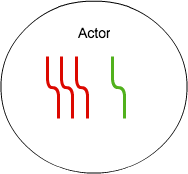
\includegraphics[scale=0.74]{mt.png}
		\caption{Basic process-oriented approach}
		\label{tp}
	\end{minipage}
	\begin{minipage}{.52\textwidth}
		\centering
		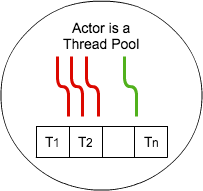
\includegraphics[scale=0.75]{atp.png}
		\caption{Actor-as-executor approach}
		\label{atp}	
	\end{minipage}
\end{figure}

\subsection{Every actor is a thread pool.}
To reduce the number of live threads in an application, we can model each invocation as a task using lambda expressions and organize each actor as a thread pool. This gives the actor an implicit queue to which tasks are submitted. We obtain a small reduction in the number of threads corresponding to the number of tasks that have been submitted, but not started. Once they are started the threads still have to compete for the actor's lock in order to execute, but the number of live threads can be restricted to the number of threads allowed by each Thread Pool, while the rest of the invocations remain in the thread pool queue as tasks. This approach is illustrated in Figure~\ref{atp}. The implementation of the four Actor features is as follows:

\begin{itemize}
	\item The actor is initialized as an object with a lock and a thread pool;
	\item Asynchronous calls are created as new threads that compete for the lock;
	\item Suspension of a call simply suspends the thread;
	\item The call stack of a synchronous call is saved in the suspended thread;
\end{itemize}




%\begin{figure}
%	\centering
%	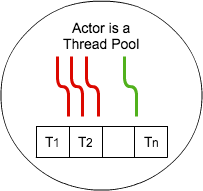
\includegraphics[scale=0.5]{atp.png}
%	\caption{Actor-as-executor approach}
%	\label{atp}	
%\end{figure}

\subsection{Every system has a thread pool.}
In the previous two approaches we modeled the concept of an actor being restricted to one task at a time by introducing a lock on which threads compete. However as all invocations are modeled as tasks that don't need a thread before they start, there is no point in starting more than one task only to have it stuck on the actor's lock. Therefore we introduce \textit{one thread pool per system} or \textit{the system's executor}, and instead of submitting the messages directly to the thread pool, we add an indirection by storing them into an explicit queue first and introduce as a second phase the submission to the thread pool. We assign a separate task for each actor to iterate through its associated queue and submit the next available message to the system thread pool. We will refer to this task from now on as the \textbf{Main Task} of an actor. This removes the requirement to store every message handler as a thread, after it starts and attempts to acquire a lock, saving a task as data in the heap instead.  However it comes at the cost of having to manage message queues manually as we need an explicit queue for all the messages that have not yet been submitted (to the thread pool). 
\par When cooperative scheduling occurs, the executing task of an actor will be suspended and therefore still live in the system as a thread so the application's live threads will be equal to the number of "await" statements in the program. The system's executor can dynamically adjust the number of available threads to run subsequent available tasks, but the application will then still be limited by the maximum number of suspended threads that can exist in the main memory. Furthermore, we still require a lock to ensure that, upon release, the suspended thread will compete with the Main Task associated to the actor from which it originated. This design is presented in Figure~\ref{stp} and it is important to observe the migration of messages into memory and that the red threads are only tasks that have been suspended by an "await". We observe the following changes in the four actor features:

\begin{itemize}
	\item The actor is initialized as an object with a lock, an explicit queue and an implementation of the \textbf{Main Task};
	\item Asynchronous calls are created as new tasks that will be run by the \textbf{Main Task} and will compete for the lock only with suspended tasks;
	\item Suspension of a call restarts the \textbf{Main Task} to iterate the actor's queue and parks the current task as a thread;
	\item The call stack of a synchronous call is still saved in the suspended thread.
\end{itemize}



%We solve the problem by using an indirection, instead of submitting the messages to the thread pool, we add an indirection by storing them into an explicit queue first and introduce as a second pahse the submission to the thread pool.


\begin{figure}
	\centering
	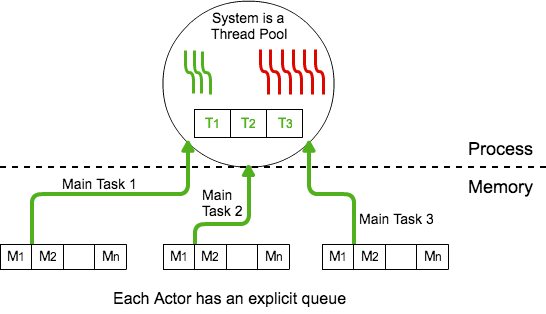
\includegraphics[scale=0.51]{stp.png}
	\caption{System as a thread pool}
	\label{stp}
	
\end{figure}

\subsection{Fully asynchronous environment.}
In the absence of synchronous calls, to eliminate the problem of having live threads when cooperative scheduling occurs, we can also use lambda expressions to turn the continuation of an await statement (which is determined by its lexical scope) into an internal method call and pass its current state as parameters to this method. Essentially what we do is allocate memory for the continuation on the heap, instead of holding a stack and context for it. We will benchmark this trade-off between the memory footprint of a native thread and the customized encoding of a thread state in memory. As there are no more suspended threads in the system to compete with the actor's Main Task, we can eliminate the lock per actor. Finally, let's consider the example in Listing~\ref{ex}. In this case the continuation consists of both the lexical scope of the release statement that is followed by the a complete synchronous call chain that has been generated(i.e. $C(m_2);C(m_1)$). The four features of the Actor are as follows:

\begin{itemize}
	\item The actor is initialized as an object with an explicit queue and an implementation of the of the \textbf{Main Task}, but without a lock;
	\item Asynchronous calls are created as new tasks that will be run by the \textbf{Main Task} and will compete for the lock only with suspended tasks;
	\item Suspension of a call first saves the continuation as a lambda expression guarded by the release condition, and the \textbf{Main Task} continues to iterate through the queue;
	\item The process of saving the call stack of a synchronous call is detailed in the next paragraph.
\end{itemize}



%In this particular scenario the simplest approach is still to save the call stack as a thread and encounter (although to a smaller extent) the same problem as in the previous paragraph. At most, we can give an increased priority to the suspended threads that save call stacks to execute on actors once they are released.
 
%If we assume a fully asynchronous environment then the continuation can always be determined by the lexical scope that follows the release statement. 
 %a separate queue of tasks that are "awaiting" either on a condition or on a future and insert it in

\paragraph{Synchronous calls context.}

In the presence of synchronous calls, the only problem that remains is how to save this call stack without degrading performance? To do this we can try to alter the bytecode to resume execution at runtime from a particular point, but we want our approach to be independent of the runtime and be extensible to other programming languages. Therefore we try to approach the problem differently; if we can turn a continuation, that does not originate from a stack of calls, into a task, is it possible to extend this to synchronous calls as well? We know that this issue arises when methods that contain an "await" statement are called synchronously, but at compile time we can easily identify all of these occurrences from the ABS code. We can simply mark them at compile time and transform them into asynchronous calls followed by an "await" statement on the future generated from the call. Now we can use the same approach for translating these continuations into tasks using lambda expressions and thus eliminating any suspended threads in the system. The final model of our solution is presented in Figure~\ref{sol}. The details of how to construct these continuations and schedule them are presented in Section~\ref{comp}. 
\par A fully asynchronous environment means to change a synchronous call \\ \lstinline|x = this.m();| into an asynchronous call plus an await like \lstinline|f = this!m();| \\ \lstinline| x = await f?;|. There are two problems here. First, we still need to make sure that "m" must be the exact next method that will run. Second, when "m" finishes, the actor scheduler must immediately schedule the method that is waiting for its result. Both can be implemented by changing the non-deterministic behavior of the Main Task. There are two constrains that we have to impose to preserve the chain of synchronous calls. First, we set a flag "isSyncCall" in the task that is calling "m" and when that flag is true, the Main Task will immediately execute the message that is to be enqueued instead of taking an arbitrary one from the queue. Second, assuming that there is no "message overtaking", the messages that are part of a synchronous call chain arrive in the Actor's queue in the FIFO order. We can label each call chain with a number "syncContext" and all messages part of that call chain will have this number. When the Main Task completes a message labeled with a particular number it will take from the queue the next available message with the same label and execute it. Finally, when the last message with that label is complete, then the call chain is complete and the next message will be selected arbitrarily.

\begin{figure}
	\centering
	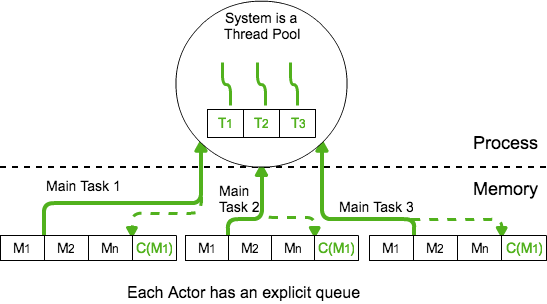
\includegraphics[scale=0.47]{solution.png}
	\caption{Full data-oriented approach}
	\label{sol}
\end{figure}

%\subsection{Optimizations for the JVM}
%\label{optimizations}
%We investigate the performance impact of eliminating the large number of expensive threads in Java that are required to implement the cooperative scheduling model. Using this data-oriented approach for saving contexts we limit any application to the system's main memory size, but added to that we also obtain some other optimizations related to Java's features.
%
%\paragraph{Demand-driven approach.}
%An important advantage of having a task assigned to each actor and a manually processed queue is that we can start and stop the task depending on the queue state. To avoid keeping the Main Task alive, we make it part of the functionality of sending a message or completing a future to notify the Main Task. This is done by any other actor who sends an invocation to an empty queue and subsequently the Main Task stops when there are no more enabled messages in the queue. This gives rise to some subtle synchronization points that will be detailed in Section~\ref{run}. An important observation to make here is the two scenarios that re-enable tasks. These release points may occur when actors fulfill a future and therefore we require the system to have a notification mechanism for actors with empty queues and newly enabled messages which we will detail in Section~\ref{run}. This requires maintaining a global hash table, mapping every future to the set of actors that are awaiting on its completion. When release points occur due to an internal state becoming valid, the Main Task is responsible for verifying the boolean condition before it may end (possibly because of no enabled messages), so no special notification is required in this case.
%
%%As ABS semantics do not allow actors to modify each other's internal state, we know that a release point that will validate a boolean condition based on a change of an actor's state can only occur during another task that is already executing on that actor. This release point will always occur before the running task ends and therefore the queue can never be empty as the released message will be available in the queue and no special notification will be required to resume the task assigned to the actor. 
%
%
%\paragraph{Optimal usage of system threads.}
%The approach of using one thread pool per system gives the user direct control over the number of live threads the application creates. Using the Executor interface in Java allows the user to choose the type of thread pool that manages the actors and set the maximum number of threads that are available. For example the user can limit the number of threads the application has to the number of cores that the machine provides and avoid context switches made by the JVM. This in turn means that the implementation has to provide fair usage of the threads with respect to the Main Tasks that run the actors, an issue which we will also touch upon in Section~\ref{run}. 
%
%\paragraph{Eliminating busy waiting.}
%Cooperative scheduling through the "await" statements may suspend the current message run by the actor based on either a particular inner state or future requiring completion on a different actor. We discussed how the Main Task can start or stop based on release points, but how exactly does an actor verify that a release point has completed? Clearly, having a task continuously iterate through all suspended messages (busy-waiting) is inefficient. While we can permanently mark a message that needs a future to complete as available, by the nature of ABS, we cannot do that for a message which is released by a particular valid state, as its state can change again by the time it is run, so it always has to be verified before it is fetched. Instead, we assign this verification to the Main Task that iterates through the queue, and simply stop the task if no message is available. If the task does stop, it means that the actor is in a state in which it is unable to execute any of its suspended messages. Therefore, it requires another actor to either send a new invocation that will change its state or the system to send a notification about a future that may release some of its messages and re-enable the Main Task. 
%
%
%\paragraph{Using JVM Garbage Collection}
%Using the approach explained so far in this section, the only extra references we need for the actors are the ones inside the global hash-table required for the notification mechanism for futures. Once the future is completed and notifications are sent, the key is deleted and the actor references become unreachable. Therefore we can leave the entire garbage collection process to the Java Runtime Environment as no other bookkeeping mechanisms are required.


%\section{Generation and Scheduling of Continuations}
\label{comp}

When cooperative scheduling occurs, the continuation must be created and then scheduled as a new task. There are two problems with that. Firstly, the continuation is not just another method, but part of it, and thus cannot just be turned into a Runnable, so that it can be enqueued. Secondly, in presence of synchronous calls, the whole stack needs to be part of the continuation and scheduled accordingly. 

%First, we assume no stack is present and try to address the first problem. Then we propose a solution to the stack issue in an orthogonal way. Theoretically, at runtime, you simply could make a pointer to the current “instruction pointer” and use it as the continuation. Of course, you need to store all the local variables. This would be a viable solution, if we could at runtime create a method whose entry point is the current (or more specifically, the next) instruction (or in terms of Java, the next bytecode instruction). This method should take as parameters, all the local variables of the currently executing method, including its parameters. Another solution is to do a preprocessing and statically create these methods.

\subsection{Preprocessing continuations at compile time}
Preprocessing of continuations can be done in both ABS or Java, but it is better to do in Java because then this code would apply also when using the proposed library directly in Java. The following explains how to do the preprocessing. The idea is that every await is replaced by a method call. For example:

\begin{lstlisting}
void m1( Int p) {
	Boolean b;
	Int i;
	while (b) {
		await this.g?; // let say this is await number 1, and assume g is a class field
		i = 0;
}	}
\end{lstlisting}

will translate to:
\begin{lstlisting}
void m1(Int p) {
	Boolean b;
	Int i;
	while (b) { 
		if (!g) {
			this ! await_1(i, b, p); 
			return;
		}
		i = 0;
}	}
\end{lstlisting}

Then we have to generate the inner method "await\_1()" or in fact one of these methods per await statement. Generation can be done using the following rules:

\begin{lstlisting}
Cont(S1;S2) = Cont(S2) IF await in S2
Cont(S1;S2) = Cont(S1);S2 IF await in S1
Cont(while(b){S}) = Cont(S); while(b){S} IF await in S
Cont(if(b) S1 else S2) = Cont(S1) IF await in S1
Cont(if(b) S1 else S2) = Cont(S2) IF await in S2
\end{lstlisting}
For the above example, we get the following:

\begin{lstlisting}
Cont(m1) = Cont(while(b) { await g; i = 0 })
= Cont(await g; i = 0); while(b) {await g; i = 0 }
= { i = 0; while(b) {await g; i = 0 } }
void await_1(Int i, Boolean b, Int p) {
	i = 0; 
	while(b) {
		if (!g) {
			this ! await_1(i, b, p);
			return;
		}
		i = 0 ;
}	}
\end{lstlisting}

\subsection{Synchronous Calls}
A fully asynchronous environment means to change a synchronous call \\ \lstinline|x = this.m();| into an asynchronous call plus an await like \lstinline|f = this!m();| \\ \lstinline| x = await f?;|. There are two problems here. First, we still need to make sure that "m" must be the exact next method that will run. Second, when "m" finishes, the actor scheduler must immediately schedule the method that is waiting for its result. Both can be implemented by changing the non-deterministic behavior of the Main Task. There are two constrains that we have to impose to preserve the chain of synchronous calls. First, we set a flag "isSyncCall" in the task that is calling "m" and when that flag is true, the Main Task will immediately execute the message that is to be enqueued instead of taking an arbitrary one from the queue. Second, assuming that there is no "message overtaking", the messages that are part of a synchronous call chain arrive in the Actor's queue in the FIFO order. We can label each call chain with a number "syncContext" and all messages part of that call chain will have this number. When the Main Task completes a message labeled with a particular number it will take from the queue the next available message with the same label and execute it. Finally, when the last message with that label is complete, then the call chain is complete and the next message will be selected arbitrarily.

%\begin{itemize}
%	\item we set a flag "isSyncCall" in the task that is calling "m" when that flag is true, it will immediately execute the message that is to be enqueued instead of taking an arbitrary one from the queue. 
%	\item Assuming that there is no "message overtaking" we know that messages that are part of a synchronous call chain arrive in the Actor's queue in a FIFO order. Therefore we can label each call chain with a number "syncContext" and all messages part of that call chain will have this number. Therefore when the Main Task completes a message labeled with a particular number it will take from the queue the next available message with the same label and execute it. Finally when the last message with that label is complete, the next message will be taken arbitrarily.
%\end{itemize}

%This change regards the implementation of the Main Task. That task will need another flag "isSynchCall" and when that flag is true, it will immediately execute the message that is to be enqueued instead of taking an arbitrary one from the queue. 

%Completion of futures

%The problem is when an actor has no enabled messages, it may only be reenabled when a future it is waiting on completes. But how should the actor be awakened in this case? The answer is by the actor who completes the future.

%There must be a global hash table, mapping every future to the set of actors that are awaiting on its completion. When a future completes (basically when a method finishes), the current actor looks up this future in this hash table, and sends a special `enable` method to all awaiting actors, and this method takes the future as the parameter. On the other side, every actor puts the messages awaiting a future into a special queue of suspended messages. The `enable` method takes the message waiting in this future and puts them to the default queue of enabled messages. Note that the messages awaiting on boolean conditions, are in separate queues as we discussed in the previous post.

%- Mahdi's blog post 

%Conceptually an actor has one thread of execution, which means it can run only one method at a time. Practically, however, allocating a real thread for each actor is highly expensive. Very roughly speaking, an executor service in Java provides a queue of tasks and an efficient way of running those tasks on a few threads. Due to the optimizations provided by Java implementations, an executor in principle is the best way to scale to many concurrent tasks. We use the terms executor and thread-pool interchangeably. There are two possibilities in how to use executors when modeling actors.

%One Task Per Message

%Conceptually, one message handler (or method) may be seen as the unit of execution — forgetting about release points and awaits for now. By submitting one task to the executor upon receiving a message, we in effect also delegate the queueing of the messages over to the executor. This is good as we may assume executors have optimized implementations for handling queues. The disadvantage here is that we will need a lock per actor that must be checked by every message handler upon start, and freed upon completion. We can reduce the number of lock-based synchronization by handling actor queues manually, as described below.

%One Task Per Actor

%From a different perspective, we may see an actor itself as a unit of execution, as in conceptually has exactly one thread. This justifies having one task in the executor thread pool per actor. This means that we must handle the message queue of each actor separately. The task corresponding to an actor is then responsible for taking messages one by one from the queue and running them. This removes the requirement to synchronize every message handler, but it comes at the cost of having to manage message queues manually.

%There is a problem when the queue is empty. Since we do not want to make this task busy-wait until a message arrives, an idea would be to check upon insertion of a new message into the queue whether such a task exists already. This again, however, requires some careful synchronization, but we expect that this is less severe than the previous case (although we cannot prove it). To do so, for every actor, we keep a local atomic boolean flag `running`. A first approach looks like this:

%// inside the task
%Runnable task = () => (
%while (!q.isEmpty()) {
%	// take one message and run it
%} 
%running.set(false);
%);
%// when inserting a new message
%q.insert(m);
%if (!running.getAndSet(true)) {
%	executor.submit(task);
%}
%The problem with the above code is that the check of the queue for emptiness and setting the flag to `false` is not atomic, and in between these two statements, a new message may be inserted into the queue without spawning a new task. To remedy this, we need to introduce a new method that can check the queue for emptiness and set the flag to `false` in a critical section, for example inside a `synchronized` block using the `q` or `running` as the lock. Additionally, either the insertion into the `q` or getAndSet of `running` should also use the same lock obviously.
%
%boolean isQueueEmptyAndReset(q, running) {
%	synchronized (running) {
%		if (q.isEmpty()) {
%			running.set(false);
%			return true;
%		} 
%		return false; 
%	}
%}
%boolean getAndSetSync(running) {
%	synchronized (running) {
%		return running.getAndSet(true);
%	}
%}
%
%// inside the task
%Runnable task = () => (
%while (!isQueueEmptyAndReset(q, running)) {
%	// take one message and run it
%} 
%);
%// when inserting a new message
%q.insert(m);
%if (!getAndSetSync(running)) {
%	executor.submit(task);
%}
%Additionally, the flexibility on controlling the queues may even be useful. We can indeed make use of this for handling release points and await statements. We suggest to use various queues for every actor, each coupled with a predicate, for example checking a boolean or completion of a future, and then at every scheduling point, one message from one of the enabled queues is taken, and executed. This is obviously assuming that when releasing the processor (e.g., via `await`) the continuation is clearly a runnable/callable that can be put into the queue.
%
%Fairness
%
%Another problem with the approach above is that (when there are more actors than available threads), some actors may keep processing one message after the other from its queue, and thus keeping the thread it is running on, while some other actors are starving, i.e., not being assigned to any thread. To remedy this, we could change the while loop to an if statement like this:
%
%// inside the task
%Runnable task = () => (
%// take one message and run it, and then ...
%if (!isQueueEmptyAndReset(q, running)) {
%	executor.submit(this);
%} 
%);
%// when inserting a new message
%q.insert(m);
%if (!getAndSetSync(running)) {
%	executor.submit(task);
%}





%- formal explanation for creating continuations.
\section{Implementation}
\label{run}
The implementation of the full data-oriented scheme is done through a library which contains a set of classes and interfaces that have a direct mapping to the ABS language concepts described in Section~\ref{lang}. The library provides an implementation of cooperative scheduling behavior, the suspension and release mechanisms while respecting the logic of synchronous calls. The library provides the solution and the optimizations discussed in Section~\ref{scheme}. The library can be obtained as a maven project and is available online~\cite{library}.



%A problem that can arise when there are more actors than available threads in the system's executor, some actors may keep processing one message after the other from its queue, and thus keeping the thread it is running on, while some other actors are starving, i.e., not being assigned to any thread.

%\subsection{Suspension and Release Points}
%To implement cooperative scheduling our library provides abstractions for guards that control suspension and release points. The are supported through the abstract class \textbf{Guard} and its subclasses \textbf{FutureGuard}, \textbf{PureExpressionGuard} and \textbf{ConjunctionGuard} that describe the conditions on which an actor's message can await: either a future, a particular valid expression or a group of these conditions respectively. 

\subsection{Actor Implementation}
The library offers an interface \textbf{Actor} containing several methods for implementing the behavior of synchronous (\textit{sendSync}), asynchronous (\textit{send}) method calls and await statements (\textit{await}) from ABS. The library currently supports an implementation of this interface called \textbf{LocalActor} for actors running on the same machine. An important advantage of having a task assigned to each actor and a manually processed queue is that we can start and stop the task depending on the queue state. To avoid keeping the Main Task alive, we make it part of the functionality of sending a message or completing a future to notify the Main Task. This is done by any other actor who sends an invocation to an empty queue and subsequently the Main Task stops when there are no more enabled messages in the queue. 

\par Inside the \textbf{LocalActor} class there is a \textit{messageQueue} defined which holds all the invocations (synchronous or asynchronous) that have been submitted to the actor as tasks. The implementation defines an inner class \textit{MainTask} which is a Java Runnable that corresponds to the task responsible for taking messages from the queue and running them. When the queue is empty, we do not want to make this task busy-wait until a message arrives, and so, upon insertion of a new message into the queue, there is a check whether such a task exists already. This gives rise to some subtle synchronization points. For every actor, we keep a local atomic boolean flag \textit{mainTaskIsRunning}. A first approach looks like in Listing~\ref{basicsync}:  \\ \\

\begin{lstlisting}[float, caption= Basic Synchronization for the Demand-Driven Approach, label=basicsync]
	// inside the task
	class MainTask implements Runnable{
		public void run() ({
				// iterate through queue and take one message and run it
			mainTaskIsRunning.set(false);
	}	}
	
	// when inserting a new message
	messageQueue.add(m);
	if (!mainTaskIsRunning.compareAndSet(false, true)) {
		DeploymentComponent.submit(new MainTask())
	}
\end{lstlisting}
\begin{lstlisting}[caption= Complete Synchronization for the Demand-Driven Approach, label=completesync]
private boolean takeOrDie() {
	synchronized (mainTaskIsRunning) {
		
		// iterate through queue and take one ready message 
		// if it exists set the next message for the main task and then
		return true;
		
		//if the queue if empty or no message is able to run
		mainTaskIsRunning.set(false);
		return false;
}	}
private boolean notRunningThenStart() {
	synchronized (mainTaskIsRunning) {
		return mainTaskIsRunning.compareAndSet(false, true);
}	}

// inside the task
class MainTask implements Runnable{
	
	public void run() {
	while (takeOrDie())
		// proceed to take the next message message and run it	 
	}	
}

// when inserting a new message
messageQueue.add(m);
if (notRunningThenStart()) {
	DeploymentComponent.submit(new MainTask());
}
\end{lstlisting}

The problem with the code in Listing~\ref{basicsync} is that the check of the queue for emptiness and setting the flag to "false" is not atomic, and in between these two statements, a new message may be inserted into the queue without spawning a new Main Task. To remedy this, in Listing~\ref{completesync}, we introduce a new method that can check the queue for emptiness and set the flag to "false" in a critical section, for example inside a "synchronized" block using the \textit{messageQueue} or \textit{mainTaskIsRunning} as the lock. Additionally, either the insertion into the \textit{messageQueue} or \textit{compareAndSet} of \textit{mainTaskIsRunning} should also use the same lock.  Another problem with this approach above is that, when there are more actors than available threads, there is no fairness policy when assigning a thread to an actor. To remedy this, we could change the while loop to an if statement like in Listing~\ref{fair}: 
\begin{lstlisting}[caption= Fairness Between Actors, label=fair]
class MainTask implements Runnable{
	public void run() {
	
		if (!takeOrDie())
			return;
		// proceed to take the next message message and run it	 
		DeploymentComponent.submit(this);
	}	
}
\end{lstlisting}



\subsection{Deployment Component}
%When release points occur due to an internal state becoming valid, the Main Task is responsible for verifying the boolean condition before it may end (possibly because of no enabled messages), so no special notification is required in this case.

In ABS there are two scenarios that re-enable tasks; an internal state of the actor is valid(i.e. a boolean condition that guard a continuation evaluates to true) or a future that guards a continuation is completed by another actor. These later release points require the system to have a notification mechanism for actors with empty queues and newly enabled messages. Therefore we maintain a global hash table, mapping every future to the set of actors that are awaiting on its completion. 

\par ABS uses the concept of \textbf{Deployment Component} to describe a system or a machine on which actors run. Therefore in our library we use this class to manage the two elements that the solution requires at the system level. The first is the system executor which currently in the library is a \textit{newFixedThreadPool} singleton \textit{ExecutorService} initialized with a fixed number of threads equal to the number of cores in the system. An actor may start a new Main Task by simply calling the static method \lstinline|submit(new MainTask())| offered by the Deployment Component. Inside the class there is also support to safely call \lstinline|shutdown()| when all the actors in the application have completed execution. The second element is the notification mechanism together with a \textit{ConcurrentHashMap} that contains mappings of futures that hold release points on actors in the system. Actors that complete a certain future can call the static method \lstinline|releaseAll(f)| to notify actors that contain messages suspended on that particular future. 

\paragraph{Eliminating busy waiting.}
Cooperative scheduling through the "await" statements may suspend the current message run by the actor based on either a particular inner state or future requiring completion on a different actor. We discussed how the Main Task can start or stop based on release points, but it is important to observe how exactly does an actor verify that a release point has completed. Having a task continuously iterate through all suspended messages (busy-waiting) is inefficient. We can separate the messages that are guarded by an incomplete future until that future completes such that the Main Task does not need to check them. Subsequently they can be put in the \textit{messageQueue} once the future guard completes. The same procedure cannot be applied for a message which is released by a particular valid state, as its state can change again by the time it is run, so it always has to be verified before it is fetched. We assign this verification to the Main Task that iterates through the queue, and simply stop the task if no message is available after one iteration. If the task does stop, it means that the actor is in a state in which it is unable to execute any of its suspended messages. Therefore, it requires another actor to either send a new invocation that will change its state or the system to send a notification about a future that may release some of its messages and re-enable the Main Task. 


\paragraph{Using JVM Garbage Collection}
Using the approach explained so far in this section, the only extra references we need for the actors are the ones inside the global hash-table required for the notification mechanism for futures. Once the future is completed and notifications are sent, the key is deleted and the actor references become unreachable. Therefore we can leave the entire garbage collection process to the Java Runtime Environment as no other bookkeeping mechanisms are required. This way we do not keep a registry of the actors like the {\ttfamily context} in Scala and Akka.





\section{Benchmarking the Implementation Schemes}
\label{bench}

\subsection{Cooperative Scheduling Benchmark}
The main problem that we encountered when implementing cooperative scheduling was saving the context of an execution and resuming from that context. To do this in Java using threads and context switches heavily limits the application to the number of native threads that can be created.  To measure the improvement provided by our Scala library features using simple example that is illustrated in Listing ~\ref{absex} which involves heavy cooperative scheduling. 

%In the
%example we have one actor containing an which receives a large
%number of messages stored in its queue. This message recursively calls
%a function that creates a stack frame after which a message is
%sent to a different Actor to run in parallel a function that computes a large number of trigonometric operations . The object is then suspended to await the
%result of this function, resulting in the requirement to save the stack frame in order to allow the next message from the queue to run
%on the actor. We varied the total number
%of messages in the object's queue to compare performance between a trivial thread based approach and our optimized solution in the Java backend for ABS. 

%\begin{figure}
%	\label{sf}
%	\centering
%	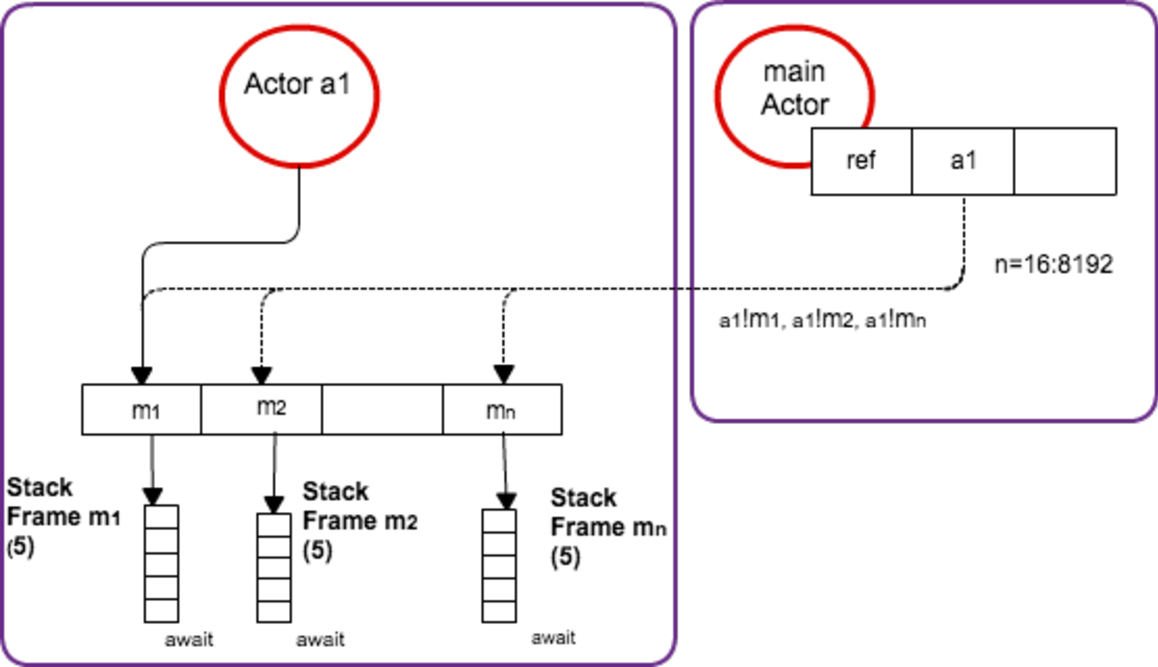
\includegraphics[scale=0.6]{scenario}
%	\caption{Cooperative Scheduling Benchmark Scenario}
%\end{figure}
%\begin{lstlisting}[caption= Benchmark Example, label=absex]
%trait Ainterface extends Actor with Ordered[Actor] {
%
%	def recursive_m( i : Int,  id : Int): Int;
%
%}
%
%class A() extends LocalActor with Ainterface {
%
%	var result : Int =  0;
%	
%	def recursive_m( i : Int,  id : Int): Int= {
%		if ((i > 0)) {
%			var msg : Callable[Int] = () => this.recursive_m((i - 1), id);
%			var future_k : ABSFutureTask[Int]  
%						= this.sendSync ((future_k_par: ABSFutureTask[Int])=>
%								this.Arecursive_mAwait0(i, id, future_k_par), msg);
%			var k : Int   = future_k.get();
%		}
%		else {
%			var msg : Callable[Int] = () => this.compute();
%			var f : ABSFutureTask[Int] = this.send (msg);
%			await(()=>this.Arecursive_mAwait1(f, i, id), Guard.convert(f), false);
%		}
%		return 1;
%	}
%	
%	def compute(): Int= {
%		result = (result + 1);
%		return result;
%	}
%	
%	def Arecursive_mAwait0( i : Int,  id : Int,  future_k : ABSFutureTask[Int]): Int= {
%		var k : Int = future_k.get();
%		return 1;
%	}
%	
%	def Arecursive_mAwait1( f : ABSFutureTask[Int],  i : Int,  id : Int): Int= {
%		return 1;
%	}
%}
\end{lstlisting}

\par The model creates an Actor of type "A" and sends a large number of messages to it to execute a method \lstinline|recursive_m(5,id)|. This method creates a call chain of size 5 before sending an asynchronous message to itself to execute a basic method \lstinline|compute()| and awaits on its result. Although simple, this example allows us to benchmark the pure overhead that arises from having a runtime system with cooperative scheduling support, both in a data-oriented approach and a process-oriented approach. The results are shown in Figure~\ref{jj}. The performance figures presented are for one actor that is running 500-2500 method invocations. It is important to observe that each invocation generates 2 messages in the actor’s queue, so as the number of calls increases the number of messages doubles. The figures show that the trade-off for storing continuations into memory instead of saving them in native threads removes limitations on the application and significantly reduces overhead. 

\begin{figure}
	\centering
	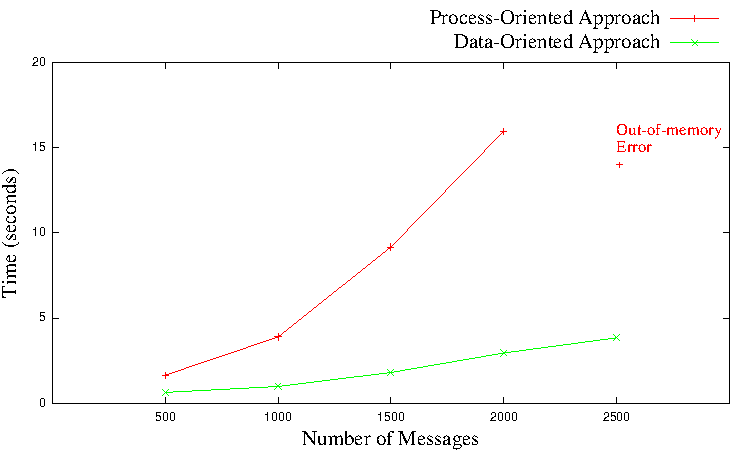
\includegraphics[scale=.68]{jaj8.pdf}
	\caption{Performance figures for pure Cooperative Scheduling}
	\label{jj}
\end{figure}

%loc
\subsection{NQueens Benchmark}
\par While our solution is catered towards a widely-used software development language, we would like to also compare with other languages that implement ABS language concepts efficiently using threads and without these limitations. In Section~\ref{run} we listed several optimizations that were inferred from our implementation solution. What we want to do is compare this optimized solution to an ABS backend implemented in Erlang that uses the same process-oriented approach but does not suffer from any limitation of native threads. We want to observe if our data-oriented approach can be comparable to Erlang's lightweight threads. For this comparison, we use the Savina benchmark for programming with actors~\cite{savina}.  We chose the problem of arranging $N$ queens on a $NxN$ chessboard as it provides a master-slave model that relies heavily on the cooperative scheduling properties of the master model.  The benchmark divides the task of finding all the valid solutions to the $N$ queens problem to a fixed number of workers that at each step have to find an intermediary solution of placing a queen $K$ on the board before relaying the message back to the master which then assigns the next job of placing queen $K+1$ to another worker. As the search space becomes smaller, w impose a threshold where the worker has to find the complete solution up to $N$ queens before sending a message back to the master. 
\par We ran the benchmark with a board size varying from 6 to 12 with a fixed number of 4 workers on a core i5 machine which supports hyper-threading. The results are shown in Figure~\ref{jj}. It is important to observe that as the board size increases, the number of solutions grows from 40 to 2680. The result in Figure~\ref{ej} show that our approach is better once the board size reaches 12 and the number of solutions to be found is 14200. This result also strengthens ABS purpose to provide a programming language for real applications.

\begin{figure}
	\centering
	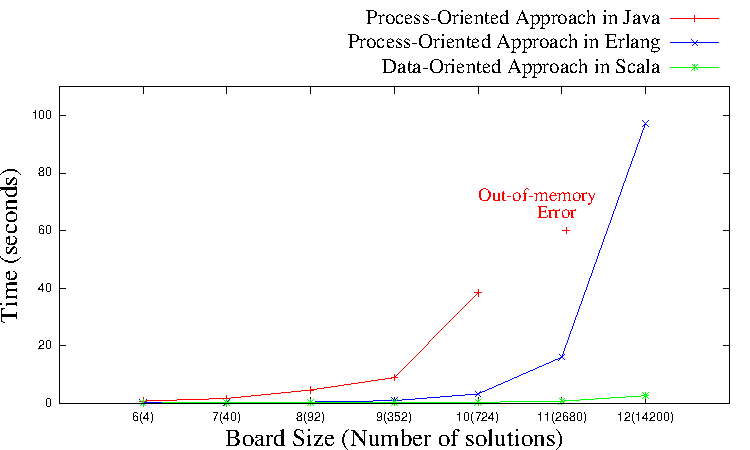
\includegraphics[scale=.7]{erlj8.pdf}
	\caption{Performance figures for the NQueens problem in Erlang and Scala Library}
	\label{ej}
\end{figure}

\par Furthermore, we would like to observe the performance impact that support for cooperative scheduling adds to an application. This feature is a powerful programming concept, but we would like to see the cost of developing a benchmark in comparison to an existing actor implementation like the Akka Actor library. We compared the implementation offered by the Savina benchmark using Akka actors with our own with a board size from 10-15 on the same machine as before. The results in Figure\ref{aj} show that the cooperative scheduling feature slows the program down by a factor of 2x, but this remains constant despite significant computation, even when the number of solutions computed reaches over 2,000,000. 

\begin{figure}
\centering
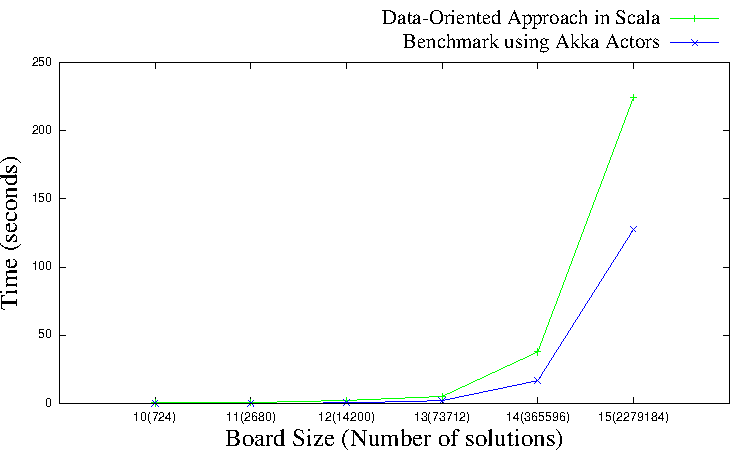
\includegraphics[scale=.7]{akka8.pdf}
\caption{Performance figures for the NQueens problem implementations in Akka and Scala Library}
\label{aj}
\end{figure}

%To measure the improvement provided by Java 8 features, we use the Savina benchmark for programming with actors~\cite{savina}.  We chose the problem of arranging $N$ queens on a $NxN$ chessboard as it provides a master-slave model that relies heavily on the cooperative scheduling properties of the master model.  The benchmark divides the task of finding all the valid solutions to the $N$ queens problem to a fixed number of workers that at each step have to find an intermediary solution of placing a queen $K$ on the board before relaying the message back to the master which then assigns the next job of placing queen $K+1$ to another worker. As the search space becomes smaller, w impose a threshold where the worker has to find the complete solution up to $N$ queens before sending a message back to the master.
% \par We benchmarked the performance of both a data-oriented approach and a process-oriented approach with 


%\par These results do show the drawback of native Java threads. However, while our solution is catered towards a widely-used software development language, it doesn't mean that there aren't other languages that are more suited to implement ABS language concepts efficiently using threads and without these limitations. In Section~\ref{optimizations} we listed several optimizations that were inferred from our implementation solution. What we want to do is compare this optimized solution to an ABS backend implemented in Erlang that uses the same process-oriented approach but does not suffer from any limitation of native threads. We want to observe if our data-oriented approach can be comparable to Erlang's lightweight threads. 






\section{Conclusions}
\label{conc}
%future work type checking
%mention debugging
In this paper we proposed a Java library for efficiently implementing the cooperative scheduling behavior of ABS which provides a powerful programming abstraction. 
To provide support for the functional data types required by ABS we embedded the Java run-time system into the Scala programming language. We showed hoe the library can be used as a design pattern to support ABS semantics. Furthermore having a portable JVM library gives us a basis for industrial adoption of the ABS language and provides ABS as a powerful extension of Scala with support for formal verification, resource analysis and deadlock detection as well as extensions that support real-time programming ~\cite{rabs}, in a software development context.

%We provided a benchmark tailored towards cooperative scheduling that show significant improvements of saving continuations including the call stack as data in memory instead of using a process-oriented approach by means native Java threads. We used a second benchmark for a CPU-intensive application to show that this feature does have a negative impact on performance compared to the Akka Actor library.

\par For future work, the ABS extension of Scala provide can be integrated with the distributed ABS implementation that exists in the Haskell backend \cite{cloud} to provide a distributed programming model for Actor-based applications.We also plan to extend the library to statically type-check the message submitted via the \textit{send} method in order to prevent the user from running unwanted code on the actors. To this end we plan to provide a syntactic sugar for an asynchronous invocation that can be used directly to send a message to an Actor.


%static type checking with respect to actor interfaces. 
%syntactic sugar 

%await the proper way

%distributed actors

%\par For future work we plan to extend the ABS typechecker to verify the Foreign Language Interface constructs directly in ABS. We also plan to develop a debugger to enable profiling and visualization of concurrent programs written in ABS. 

%We have used the library in modeling real case studies such as the auctioning agent system presented by Dastani and Testerink \cite{bas16}  or applications that already use the formal description capabilities of ABS such as the work of Hahnle and Muschevici in validating railway systems\cite{railway}.


%We have a java library
%We have already benchmarked overhead, but we want to use it for real case studies auctioning and incremental evaluation of railway systems
%Promising candidate fo a basis for industrial adoption of the ABS language.
%Advantage 
%ABS is a rich language with this backend because of the formal analysis, resource analysis and deadlock detection.
%Fromally defined language which provides the use of FA. 
%Extensions for real-time programming and distributed programming.  
%Scala backend for ABS have a full implementation of the functional data types (auctioning system)


%% Acknowledgments
\begin{acks}                            %% acks environment is optional
                                        %% contents suppressed with 'anonymous'
  %% Commands \grantsponsor{<sponsorID>}{<name>}{<url>} and
  %% \grantnum[<url>]{<sponsorID>}{<number>} should be used to
  %% acknowledge financial support and will be used by metadata
  %% extraction tools.
  Partly funded by the EU project FP7-612985
  \textsc{UpScale}: From Inherent Concurrency to Massive Parallelism
  through Type-based Optimizations \\ (\texttt{http:/$\!$/www.upscale-project.eu}). We would like to thank the reviewers for the time and effort to provide a critical and constructive review to this paper.
\end{acks}


	
%	\bibitem{Akka}  Munish K. Gupta:  Akka Essentials. Packt Publishing. p. 334. ISBN 1849518289, 2012.
%
%	\bibitem{Scala} Philipp Haller, Martin Odersky:
%	Scala Actors: Unifying thread-based and event-based programming. Theor. Comput. Sci. 410(2-3): 202-220 (2009)
%	
%	\bibitem{Sirjani} Marjan  Sirjani, Ali Movaghar:
%	An actor-based model for formal modelling of reactive systems: Rebeca.
%	Technical Report. 2001.
%	
%	\bibitem{Agha}  Gul Agha: Actors: A model of concurrent computation in distributed systems. Massachusetts Institute of Technology Cambridge Artificial Intelligence Lab.
%	1985.
%	
%	\bibitem{Schafer} Jan Sch\"{a}fer:  A Programming Model and Language for Concurrent and Distributed Object-Oriented Systems. 
%	Dissertation. University of Kaiserslautern, 2010. 
%	
%	\bibitem{KeY}Din, C. C., Bubel, R., and Hähnle, R. (2015, August). KeY-ABS: a deductive verification tool for the concurrent modelling language ABS. In International Conference on Automated Deduction (pp. 517-526). Springer International Publishing.
%	
%	\bibitem{Erlang}
%	Georg G\"{o}ri, Einar Broch Johnsen, Rudolf Schlatte, Volker Stolz:
%	Erlang-Style Error Recovery for Concurrent Objects with Cooperative Scheduling. ISoLA (2) 2014: 5-21.
%	
%	\bibitem{Haskell} 	Elvira Albert, Nikolaos Bezirgiannis, Frank S. de Boer, Enrique Martin-Martin:
%	A Formal, Resource Consumption-Preserving Translation of Actors to Haskell. 
%	Proceedings LOPSTR 2016.
%	
%	\bibitem{Encore}
%	Stephan Brandauer, Elias Castegren, Dave Clarke, Kiko Fernandez-Reyes, Einar Broch Johnsen, Ka I Pun, Silvia Lizeth Tapia Tarifa, Tobias Wrigstad, Albert Mingkun Yang:
%	Parallel Objects for Multicores: A Glimpse at the Parallel Language Encore. SFM 2015: 1-56
%	
%	\bibitem{Albert}
%	Elvira Albert, Frank S. de Boer, Reiner Hähnle, Einar Broch Johnsen, Rudolf Schlatte, Silvia Lizeth Tapia Tarifa, Peter Y. H. Wong:
%	Formal modeling and analysis of resource management for cloud architectures: an industrial case study using Real-Time ABS. Service Oriented Computing and Applications 8(4): 323-339 (2014).
%	
%	\bibitem{deadlock}
%	Elena Giachino, Cosimo Laneve, Michael Lienhardt:
%	A framework for deadlock detection in core ABS. Software and System Modeling 15(4): 1013-1048 (2016)
%	
%	
%	\bibitem{rabs}Joakim Bjork, Frank S. de Boer, Einar Broch Johnsen, Rudolf Schlatte, Silvia Lizeth Tapia Tarifa:
%	User-defined schedulers for real-time concurrent objects. ISSE 9(1): 29-43 (2013)
%	
%	\bibitem{cgf}De Boer, Frank S., Dave Clarke, and Einar Broch Johnsen. "A complete guide to the future." European Symposium on Programming. Springer Berlin Heidelberg, 2007.
%	
%	\bibitem{paj8} Nobakht, Behrooz, and Frank S. de Boer. "Programming with actors in Java 8." International Symposium On Leveraging Applications of Formal Methods, Verification and Validation. Springer Berlin Heidelberg, 2014.
%	
%	\bibitem{bas16} Mehdi Dastani, Bas Testerink:
%	Design patterns for multi-agent programming. IJAOSE 5(2/3): 167-202 (2016)
%	
%	\bibitem{abs} Johnsen, Einar, Reiner Hähnle, Jan Schäfer, Rudolf Schlatte, and Martin Steffen. "ABS: A core language for abstract behavioral specification." In Formal Methods for Components and Objects, pp. 142-164. Springer Berlin/Heidelberg, 2012.
%	
%	\bibitem{cog} Nobakht, B., de Boer, F. S., Jaghoori, M. M., and Schlatte, R. (2012, March). Programming and deployment of active objects with application-level scheduling. In Proceedings of the 27th Annual ACM Symposium on Applied Computing (pp. 1883-1888). ACM.
%	
%	\bibitem{saco} Albert, Elvira, Puri Arenas, Antonio Flores-Montoya, Samir Genaim, Miguel Gómez-Zamalloa, Enrique Martin-Martin, Germán Puebla, and Guillermo Román-Díez. "SACO: static analyzer for concurrent objects." In International Conference on Tools and Algorithms for the Construction and Analysis of Systems, pp. 562-567. Springer Berlin Heidelberg, 2014.
%	
%	\bibitem{envisage} Albert, Elvira, Frank de Boer, Reiner Hähnle, Einar Broch Johnsen, and Cosimo Laneve. "Engineering virtualized services." In Proceedings of the Second Nordic Symposium on Cloud Computing \& Internet Technologies, pp. 59-63. ACM, 2013.
%	
%	\bibitem{dead}Flores-Montoya, Antonio E., Elvira Albert, and Samir Genaim. "May-happen-in-parallel based deadlock analysis for concurrent objects." Formal Techniques for Distributed Systems. Springer Berlin Heidelberg, 2013. 273-288.
%	
%	\bibitem{dis}Serbanescu, Vlad, Keyvan Azadbakht, and Frank de Boer. "A java-based distributed approach for generating large-scale social network graphs." Resource Management for Big Data Platforms. Springer International Publishing, 2016. 401-417.
%	
%	\bibitem{cloud} Bezirgiannis, Nikolaos, and Frank de Boer. "ABS: a high-level modeling language for cloud-aware programming." International Conference on Current Trends in Theory and Practice of Informatics. Springer Berlin Heidelberg, 2016.
%	
%	\bibitem{agent_auction}Franco Zambonelli, Nicholas R. Jennings, Michael Wooldridge. 
%	Organisational Abstractions for the Analysis and Design of Multi-agent Systems
%	Agent-Oriented Software Engineering. Volume 1957 of the series Lecture Notes in Computer Science pp 235-251
%	
%	\bibitem{creol} Johnsen, Einar Broch, Olaf Owe, and Ingrid Chieh Yu. "Creol: A type-safe object-oriented model for distributed concurrent systems." Theoretical Computer Science 365.1-2 (2006): 23-66.
%	
%	\bibitem{resume} Johnsen, Einar Broch, Olaf Owe, and Eyvind W. Axelsen. "A run-time environment for concurrent objects with asynchronous method calls." Electronic Notes in Theoretical Computer Science 117 (2005): 375-392.
%	
%	\bibitem{takka} He, Jiansen, Philip Wadler, and Philip Trinder. "Typecasting actors: from Akka to TAkka." Proceedings of the Fifth Annual Scala Workshop. ACM, 2014.
%	\bibitem{execserv} https://docs.oracle.com/javase/8/docs/api/java/util/concurrent/ExecutorService.html
%	
%	\bibitem{railway}Hahnle, Reiner, and Muschevici, Radu (2016, October). Towards incremental validation of railway systems. In International Symposium on Leveraging Applications of Formal Methods (pp. 433-446). Springer International Publishing.
%	
%	\bibitem{savina} Imam, Shams., and Sarkar, Vivek. (2014). Savina-an actor benchmark suite. In 4th International Workshop on Programming based on Actors, Agents, and Decentralized Control, AGERE.


%% Bibliography
\bibliographystyle{ACM-Reference-Format}
\bibliography{bibliography}

%\begin{thebibliography}{4}
%\bibitem{library}https://github.com/vlad-serbanescu/abs-api-cwi.git
%\bibitem{lambdas} https://docs.oracle.com/javase/tutorial/java/javaOO/lambdaexpressions.html
%\bibitem{crisp} https://github.com/CrispOSS/jabsc
%\end{thebibliography}

%% Appendix

\end{document}
